\section{Testes com utilizadores}

Nos dias 18 e 19 de Julho de 2007, foram efectuados testes de usabilidade
do sistema na cidade de Glasgow, na Esc�cia.

A configura��o em uso durante o teste foi a Matrox e um microfone wireless
da Microsoft. Foram efectuados testes com 10 utilizadores, sendo os testes
efectuados em grupos de 2 utilizadores a executar as mesmas tarefas 
separadamente e uma tarefa colaborativa onde os 2 utilizadores
participaram em simult�neo, estando um deles munido dos marcadores
descritos.

%Dada a origem dos diferentes utilizadores (7 escoceses, 2 ingleses e 1 espanhol), verificou-se dificuldade em alguns deles em emitir comandos de voz correctamente reconhecidos pelo sistema.

% O arranque das ac��es com gestos necessitou de algumas tentativas. Em particular, o utilizador n�o marcado foi aconselhado a afastar-se durante o tracking.

A leitura dos marcadores mostrou-se problem�tica em pessoas de baixa estatura, tendo inviabilizado a tarefa de voo para um utilizador ap�s 3 tentativas falhadas.
Em indiv�duos altos n�o houve qualquer problema de tracking, o que leva a supor que os problemas ocorridos derivaram de oclus�es.

\begin{figure}[!h]
\centering
   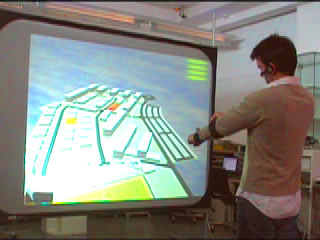
\includegraphics[width=.95\linewidth]{don.png}
 \caption{Teste em Glasgow com Utilizador em modo Voo}
\label{fig:usertest}
\end{figure}

\subsection{An�lise}

Os utilizadores estranharam por vezes a utiliza��o dos comandos "begin" e "stop". As alternativas "begin" / "end" ou "start" / "stop" seriam as mais l�gicas.
No entanto os autores haviam testado estas possibilidades durante os primeiros testes de voz, tendo-se ent�o conclu�do que "start" / "stop" eram confundidos entre si pelo motor e que "end" dava falsos positivos.

Foi sugerida a altera��o de "stop x" para simplesmente stop. Um utilizador em apuros na interac��o n�o consegue por vezes recordar o contexto em que est�, de modo a invocar o stop adequado.

Os utilizadores de modo geral ficaram agradados com as funcionalidades fornecidas por gestos + voz e n�o se mostraram inibidos na sua aplica��o.